\documentclass[a4paper,oneside,twocolumn,notitlepage,dvipdfmx]{jsarticle}
\usepackage[utf8]{inputenc}
\usepackage{amsmath}
\usepackage{amsfonts}
\usepackage{amssymb}
\usepackage{makeidx}
\usepackage{graphicx}
\usepackage{color}
\usepackage{sample}
\usepackage{url}
\usepackage{listings,jlisting}
\setlength\abovecaptionskip{1pt}
\def\baselinestretch{0.3}


\lstset{
  basicstyle={\ttfamily},
  identifierstyle={\small},
  commentstyle={\smallitshape},
  keywordstyle={\small\bfseries},
  ndkeywordstyle={\small},
  stringstyle={\small\ttfamily},
  frame={tb},
  breaklines=true,
  columns=[l]{fullflexible},
  numbers=left,
  xrightmargin=0zw,
  xleftmargin=3zw,
  numberstyle={\scriptsize},
  stepnumber=1,
  numbersep=1zw,
  lineskip=-0.5ex
}

% 以下内容

\student{谷澤 悠太}
\date{令和6年1月18日}
\prof{滝沢 寛之}
\title{中間報告}
%\author{Maohua Zhu, Tao Zhang, Zhenyu Gu, Yuan Xie}
%\journal{MICRO-52, October 12-16, 2019, Columbus, OH, USA}
\nendo{令和5年度}
 
\begin{document}
\maketitle
\section{背景・課題}
HPCは現在,機械学習や数値シュミレーション,統計解析など様々な科学分野で利用されているため,HPC利用の需要は年々高まってきている.そのため,HPCを専門としない科学者がHPCを利用する事例や情報系学生などがHPCを用いた並列計算を学習する際に利用するといった事例が多く存在する.しかしながら,このような事例の場合,HPCの利用においてシェルを用いたコマンドラインインタフェースやSSHの鍵設定などによるセットアップの複雑さ,ジョブスケジューラごとに異なる操作方法などが初学者にとって大きな障害となり得る.このように,HPCを使いこなすための前提知識は幅広く,学習コストも大きいため,HPC利用者が本来のタスクに費やすコストが減少してしまうといった問題がある.\par


\section{先行研究}
\subsection{Open OnDemand}
米国オハイオ・スーパーコンピューティングセンターはHPC利用者の支援を目的とする『Open OnDemand』(OOD)と呼ばれるオープンソースソフトウェアを開発した\cite{citation_2}\cite{citation_3}\cite{citation_4}\cite{citation_5}.OODはWebポータル上からHPCシステムの利用を可能としており,コマンドラインインタフェースではなくグラフィカルユーザインタフェースで操作することが可能なため,初学者に寄り添ったHPC利用環境を提供することができる.また,ユーザ情報の登録によるシングルサインオン認証を用いることで,誰でも環境構築を行わずに利用することが可能となっている.開発当時のOODはSLURM,Torque,PBS Pro,LSFなどのジョブスケジューラに対応していたため,現在OODを導入している計算センターも多く存在する.しかしながら,対応していないスケジューラも多く,使える環境が限定されているといった懸念点も考えられる.\par
そこで先行事例として,OODをFujitsu\_TCS(スーパーコンピュータ富岳で運用されているジョブスケジューラ)へ対応させたことによる『富岳』でのOOD利用という事例を考える\cite{citation_1}.これにより,『富岳』の利用者はHPCシステムの視覚的理解が容易になり,利用難易度が低下したというメリットを得ることができた.また,Fujitsu\_TCSのアダプタの開発により,Fujitsu\_TCSを利用している他の計算センターでもOODの利用が可能となったというメリットも挙げられる.\par

\subsection{PSI/J}
『PSI/J(Portable Submission Interface for Jobs)』\cite{citation_6}は様々なHPCのジョブスケジューラに対してHPCシステムとの統合的なインタフェースの役割を果たす.つまり,PSI/Jはスケジューラの抽象化レイヤーとして機能し,スケジューラの種類に依らずジョブの投入や削除などの一元管理が可能となる.実際に,Parsl,RADICAL-Pilot,Swift/TなどのライブラリやフレームワークはすでにPSI/Jに対応しており,その利点を十分に享受している.また,PSI/JはSLURMやLSF,PBS Pro,cobaltなどに対応しているが,OODと同様にこれらも数あるジョブスケジューラのうちの一つであり,未対応スケジューラには使用することができないといった懸念点が考えられる.

\section{目的・提案手法}
そこで本研究では『ウェブインタフェースを介したスーパーコンピュータ利用環境に関する研究』という題目を研究テーマとして考えていく.具体的には,OODとPSI/Jを通じて東北大学で用いられているスーパーコンピュータ『AOBA』の利用環境について考える.前述の通り,OODやPSI/Jはいくつかのジョブスケジューラに対応しているが,『AOBA』に用いられているジョブスケジューラNQSV(Network Queuing System V)には未対応である.そこで,ユーザとHPCシステムのインタフェースとしてOODを用いることで,HPCシステム操作方法の簡易化に伴う利用難度の低下を試みる.さらに,OODとHPCシステムのジョブスケジューラのインタフェースとしてPSI/Jを用いることで,ジョブスケジューラの仕様が異なるために発生するジョブスケジューラ依存の問題をPSI/Jに役割の細分化を図る.\par
そのため,本研究では『AOBA』の利用環境を想定しているため,図\ref{fig1}に示すようなシステムを想定している.OODが動作しているサーバとジョブスケジューラが動作するサーバは別マシンであり,HPCシステムの利用に用いられるActive Directory(AD)も独立したサーバとして稼働している.OODは各スケジューラに定義された関数を用いてジョブの管理を行っていたが,この工程にPSI/Jで用いられている各メソッドを用いることでOODはどのスケジューラに対してもPSI/Jのメソッドを用いることになり,PSI/Jがスケジューラに依存したコマンドの相違などを解消することになる.したがって,実装は大きく分けて,PSI/JのNQSV対応,OODのPSI/J対応の2つが挙げられる.\par

\begin{figure}[h]
  \centering
  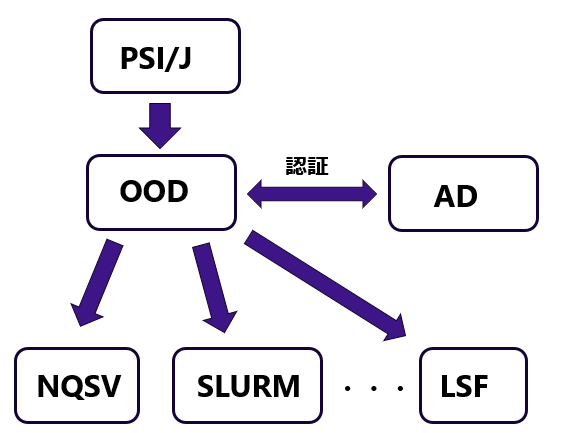
\includegraphics[width=75mm]{//home/gp.sc.cc.tohoku.ac.jp/tanizawa/study_session/2022/3rd_latex/preprint/20240118/fig/fig1.png}
  \caption{『AOBA』の仮想利用環境}
  \label{fig1}
\end{figure}



\section{進捗}
\subsection{PSI/J⇔NQSVの接続}
まず始めにPSI/JとNQSVの接続を考える.PSI/Jにはジョブの投入や削除などを行うJobExecutorクラスと対象のジョブ自身を表すJobクラスなど複数のクラスとメソッドで構成されている.特に,JobExecutorクラスは選択するスケジューラごとにサブクラスが構成され,PSI/Jは現在SLURMやPBS Pro,LSFなどに対応しているため,それぞれ個別のJobExecutorクラスが存在している.\par
今回はNQSVとの接続を実装するため,NQSV用のExecutorクラスを作成することを目指す.Executorクラスには大きく分けて3つの動作を行う関数が定義されていて,ジョブの投入,ジョブの削除,ジョブのステータスの取得を行うメソッドが定義されている.\par
まず始めに,ジョブの投入を行うメソッドを作成した.ジョブ投入に関するメソッドはNQSVの前身であるPBS ProのJobExecutorの内部とほとんど変わらずに作成することができたが,PBS Proと異なり,NQSVでは投入するキューを明示的に指定しなければジョブを投入できないといった特徴があるため,ジョブスクリプトを作成するために用いられるスクリプト中でキューの指定を行うための「\#PBS -q execque1」という行を挿入する必要があった.\par
続いて,ジョブのステータスを取得するメソッドを作成した.前述の通り,大半の構成はPBS Proとほとんど同じだが,大きく異なる点として両者のqstatの仕様の違いが挙げられる.PBS Proではqstatコマンドに-xオプションを付けることで実行が完了した過去のジョブのステータスも確認することができ,得られたステータスからジョブの完了を認識することができたが,NQSVでは終了してしまったジョブはqstatコマンドでステータスを確認することができないため,ジョブの完了を示すステータスがそもそも存在しない.そのため現在,PSI/J⇔NQSVでは完了したジョブにCOMPLEATEDのステータスをマッピングすることができていない状態になっており,実際にはジョブが完了しているのにもかかわらず,ジョブの投入中を示すQEAEADのステータスが永続的に割り振られている.この状態を避けるためにqstatコマンドを投げて出力がかえって来ない場合にCOMPLEATEDステータスを割り振るなどのアイデアがあるが現段階では未実装である.\par
最後にジョブの削除を行うメソッドを作成した.ジョブの削除に関しても構成はほとんどPBS Proと同じものであるが,PBS Proではジョブが削除された際に返される終了コードの値を用いてジョブが正常終了したかコマンドにより削除されたのかを判別していたが,NQSVではPBS Proにおける終了コードの役割を果たすものが存在しないと考えられる.そのため,NQSVではキューに入っていないジョブに対してステータスがCOMPLETEDの状態であるのかCANCELEDの状態であるのか区別することができなくなってしまっている.\par
先に示した三つのメソッドをテストした.実行コードと出力結果を図\ref{fig2},図\ref{fig3}に示す.図\ref{fig2}ではNQSVのExcutorクラスを作成した後,テスト用に用いられている実行スクリプトを用いて標準出力先とエラー出力先を指定したJobクラスを作成し,submitメソッドを実行した後とcancelメソッドを実行した後にqstatコマンドの出力結果を表示した.これにより,各メソッド後のキュー内部のジョブの状態を観測することができる.図\ref{fig3}より結果を確認すると確かにsubmitメソッド後はジョブが投入されているのに対してcancelメソッド後はキューの中身が何も入っていないことがわかり,PSI/J⇔NQSVの実装が予想通りに動作していることがわかる.なお,テスト結果のSTTで示されているステータスPRRはジョブの実行前処理中を表すステータスである.

\begin{figure}[h]
  \centering
  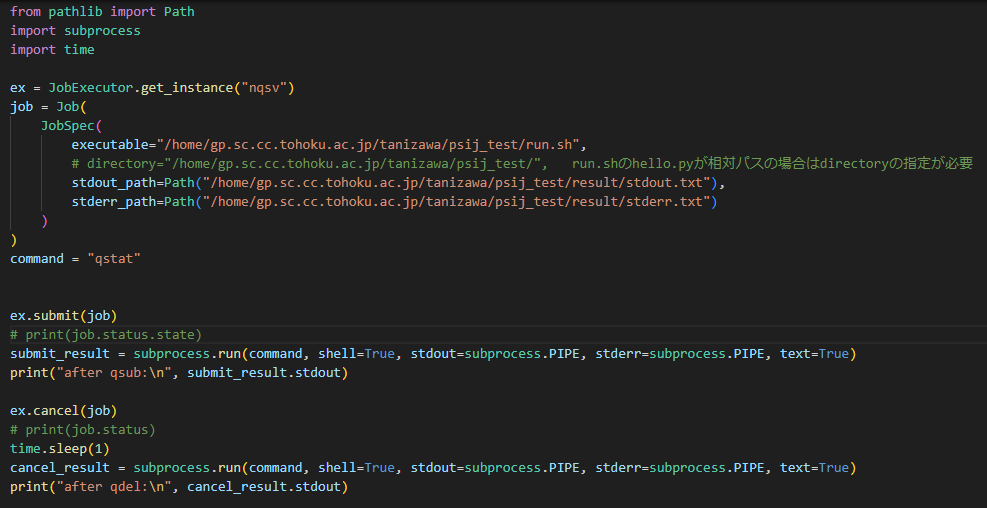
\includegraphics[width=75mm]{//home/gp.sc.cc.tohoku.ac.jp/tanizawa/study_session/2022/3rd_latex/preprint/20240118/fig/fig2.png}
  \caption{テスト実行コード}
  \label{fig2}
\end{figure}

\begin{figure}[h]
  \centering
  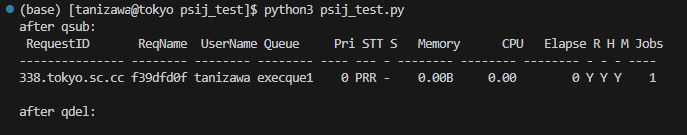
\includegraphics[width=75mm]{//home/gp.sc.cc.tohoku.ac.jp/tanizawa/study_session/2022/3rd_latex/preprint/20240118/fig/fig3.png}
  \caption{テスト出力結果}
  \label{fig3}
\end{figure}

\subsection{OOD⇔PSI/Jの接続}
続いてOODとPSI/Jの接続を考える.設計としてOODのジョブの投入や削除を行う各メソッドからそれぞれ役割を果たすためのPSI/Jメソッドを呼び出すことができるようにしたい.これにより,ユーザの依頼を受けたOODはスケジューラに直接命令を出すのではなく,PSI/Jを仲介して命令を送ることになり,前章で示した,スケジューラの抽象化機構を挟むことができる.また,この実装の中で,OODがRubyスクリプトで記述されているのに対して,PSI/Jはpythonで記述されているため,個々のメソッド用のスクリプトを書き,OODが作成されたpythonスクリプトを必要に応じて呼び出すといった形式をとる.\par
現在はOOD⇔PSI/Jでのsubmitメソッド,cancelメソッドのの実装途中である.OOD上のJobComposerでsubmitボタンをクリックするとPSI/J経由でジョブが投入されるようになったが,図\ref{fig4}に示すように,OOD内部でJobのパスを明示しないと動作しない状態であり,様々なジョブを選択して実行することができていない.submitメソッドは引数がOOD内で定義されているScriptクラスのインスタンスであるため,このScriptクラスからジョブスクリプトのパスを得ることができれば正常に動作する.\par
また,ジョブの削除を行うdeleteメソッドも実装途中であり,submitメソッドと同様にOODによって与えられる引数とPSI/Jのsubmitメソッドを行うために必要な引数が違うために問題が生じている.図\ref{fig5}に示すように,引数にはidのみが与えられるが,ジョブの削除をPSI/Jで行うためにはPSI/Jで定義されるJobクラスの情報が必要なため,submitメソッドをPSI/Jで実行した際に,用いたJobクラスのデータを残しておき,deleteメソッドの実行時に与えられたidと一致するidをもつJobクラスを取り出す必要がある.現在は,Pythonスクリプト間でJobクラスを受け渡す機能の実装中である.\par 

\begin{figure}[h]
  \centering
  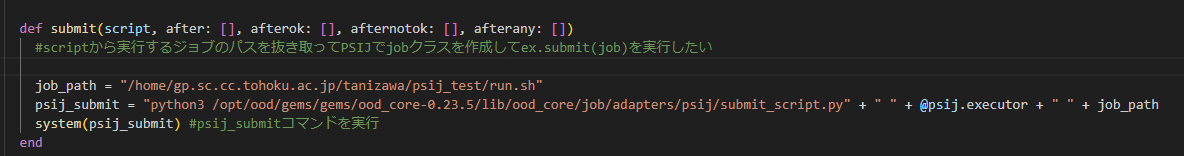
\includegraphics[width=75mm]{//home/gp.sc.cc.tohoku.ac.jp/tanizawa/study_session/2022/3rd_latex/preprint/20240118/fig/fig4.png}
  \caption{OODのsubmitメソッド}
  \label{fig4}
\end{figure}

\begin{figure}[h]
  \centering
  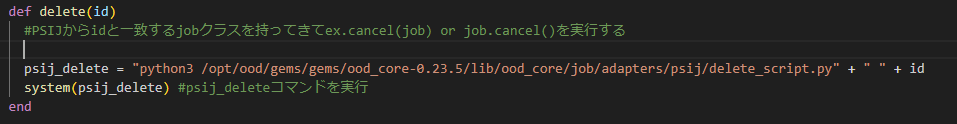
\includegraphics[width=75mm]{//home/gp.sc.cc.tohoku.ac.jp/tanizawa/study_session/2022/3rd_latex/preprint/20240118/fig/fig5.png}
  \caption{OODのdeleteメソッド}
  \label{fig5}
\end{figure}

\section{今後の予定}
来週までに,\par
・OOD⇔PSI/Jでのsubmitメソッド,cancelメソッドのの実装\par
短期目標として,\par
・OOD⇔PSI/Jでのqstatメソッドの実装\par
・OOD⇔PSI/Jの動作確認\par
中長期目標として,\par
・本番発表用の前刷り・スライドの作成\par
を考えている.\par

\bibliographystyle{junsrt}
\bibliography{refer}

\end{document}